\chapter{Scientific Background}
\label{chap:scientific_background}
This chapter provides a theoretical background for the topics addressed in this thesis.
It introduces the fundamental physical processes and structures of Active Galactic Nuclei (AGN), with a particular focus on the properties of the Broad-Line Region (BLR), which plays a central role in this work. The concept of AGN unification, the different observational classifications, and the variability of AGN are outlined.Furthermore, reverberation mapping is discussed in detail, as it serves as the main analysis method in this thesis. It is a powerful tool to probe the geometry and kinematics of the BLR and to estimate the mass of the central supermassive black hole.In the final section of this chapter, an overview of Bowen fluorescence is provided, as this process may account for some spectral features that will be discussed in the following analysis.

\section{Active Galactic Nuclei}
\label{sec:agn}

What are Active Galactic Nuclei (AGN)? They represent a class of galaxies that are among the brightest and most energetic objects in the known universe, with bolometric luminosities ranging from $10^{41}$ to $10^{48} \ \mathrm{erg \ s^{-1}}$, surpassing typical galaxies by many orders of magnitude \parencite{peterson1997introduction}.\
This enormous emission originates from the central region of the AGN, which outshines the stars of its so-called host galaxy. It is powered by matter accreting onto the central supermassive black hole (SMBH) in the form of an accretion disk \parencite{shakura1973black}.\\
To better understand the physical nature of AGN, it is important to examine their observational characteristics and internal structure. AGN emit radiation across the entire electromagnetic spectrum, and their spectral features provide crucial information about the physical conditions and kinematics in the central regions.\\
The following sections present the main components of AGN, introduce the unification model that links different AGN types, and describe commonly used classification schemes. Particular attention is given to the variability of AGN, which plays a central role in the reverberation mapping analysis carried out in this thesis.


\subsection{Structure of an AGN}
\label{sec:agn_structure}

The structure of an AGN consists of several distinct components, as illustrated in Figure \ref{fig:agn_structure_mo}. These include a central supermassive black hole (SMBH), an accretion disk that feeds the SMBH, a surrounding dusty torus, and ionized gas regions known as the broad-line region (BLR) and narrow-line region (NLR). In some AGNs, powerful relativistic jets are launched perpendicular to the accretion disk. However, these jets will not be discussed further in this section, as they are not relevant to the scope of this thesis. Each of the components contributes differently to the observed spectrum of the AGN, as will be discussed in more detail in Section \ref{sec:spectral_features}.


\begin{figure}[!ht]
	\centering
	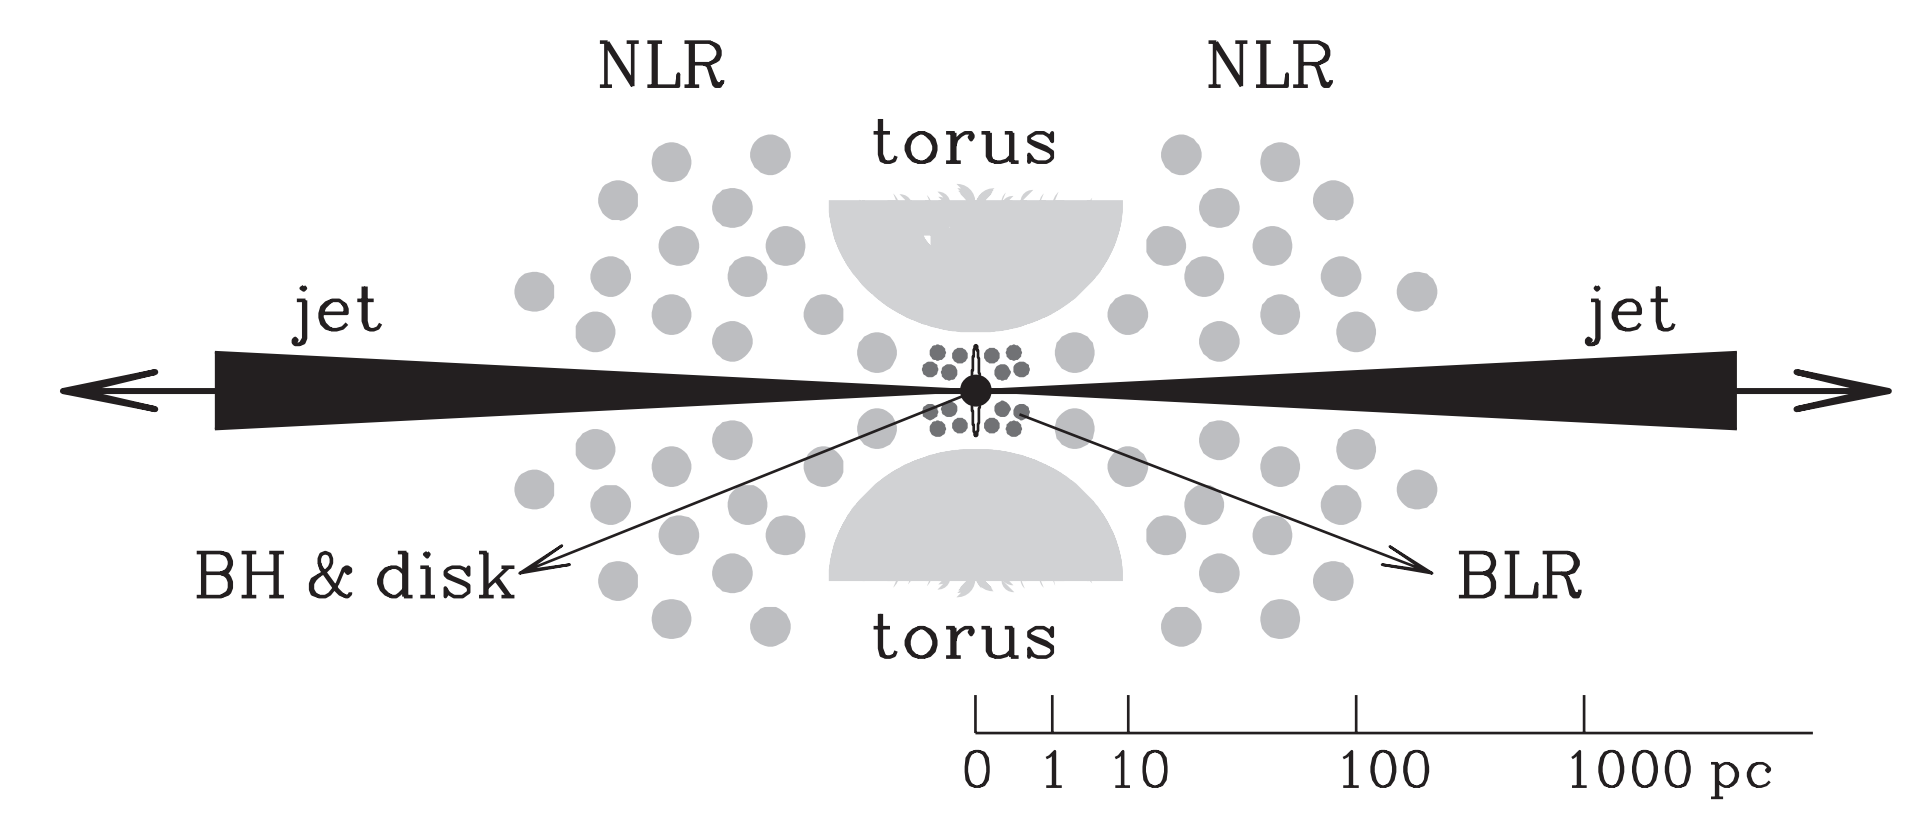
\includegraphics[width=0.8\textwidth]{pictures/Chapter2/AGN_standard_paradigm.png}
	\caption{Different components of an AGN. Adapted from \textcite{mo2010galaxy} Figure 14.3.}
	\label{fig:agn_structure_mo}
\end{figure}

\subsubsection{Supermassive Black Hole and Accretion Disk}


The center of an AGN is occupied by a supermassive black hole (SMBH), with masses typically ranging from $10^6\,M_\odot$ to more than $10^{10}\,M_\odot$. While the SMBH itself does not emit radiation, it dominates the gravitational potential in the innermost regions and acts as the central engine driving all observed AGN phenomena. Gas from the surrounding accretion disk slowly spirals inward toward the SMBH due to angular momentum transport driven by viscosity inside the disk. During this process, gravitational potential energy is converted into heat, causing the disk to reach very high temperatures. As a result, a significant fraction of the gravitational energy of the matter is transformed into thermal radiation, which accounts for the enormous luminosity observed in AGNs \parencite{netzer2013agn}.\\
The accretion disk itself is a geometrically thin and optically thick structure composed of ionized gas in differential rotation around the SMBH \parencite{shakura1973black}. The disk's composition is primarily ionized hydrogen and helium, with traces of heavier elements \parencite{netzer2013agn}. It extends from the innermost stable circular orbit (ISCO) near the event horizon out to distances of several light-days, where the temperature drops and dust can survive. The radial extent of the disk is relatively small on galactic scales, typically ranging from a few light-hours to a few light-days, corresponding to about $10^{-3}$ to $10^{-2}$\,pc \parencite{netzer2013agn,hickox2018obscured}.  The hottest regions are located in the innermost part of the disk, with typical temperatures ranging from $10^4$ to $10^5$\,K \parencite{hickox2018obscured}. 


\subsubsection{Broad-Line and Narrow-Line Region}

Outside the accretion disk lies a distribution of photoionized gas clouds that give rise to the characteristic emission lines observed in AGN spectra. The innermost of these is the broad-line region (BLR), located at distances of a few light-days to light-weeks from the central SMBH. The BLR consists of dense gas clouds (electron densities $n_e \sim 10^9$–$10^{11}\,\mathrm{cm}^{-3}$) moving at high velocities of several thousand kilometers per second due to the strong gravitational influence of the black hole \parencite{netzer2013agn}. These velocities lead to significant Doppler broadening of permitted emission lines and line widths of several thousand km/s. The BLR is primarily photoionized by the continuum radiation emitted from the accretion disk.\\
Further out lies the narrow-line region (NLR), which extends over scales of hundreds to thousands of parsecs. The gas in this region is less dense ($n_e \sim 10^2$–$10^6\,\mathrm{cm}^{-3}$) and moves at much lower velocities (a few hundred km/s), resulting in narrow emission lines with widths typically below $1000\,\mathrm{km/s}$. In contrast to the BLR, the NLR emits both permitted and forbidden lines, which gets excited by collision and can only form in low-density environments. The NLR is often spatially resolved in nearby AGNs and is photoionized by the central source, although additional ionization from shocks may also contribute in some cases \parencite{hickox2018obscured,netzer2013agn}.\\
Both the BLR and NLR serve as important diagnostics of the AGN structure and provide key information about gas dynamics, ionization mechanisms, and the orientation-dependent appearance of the active nucleus.



\subsubsection{Dusty Torus}

Surrounding the accretion disk and broad-line region is the dusty torus, a geometrically thick and optically dense structure composed of gas and dust. It extends from the sublimation radius, where dust can survive the intense radiation of the accretion disk, out to scales of a few parsecs. The torus likely has a clumpy distribution and plays a crucial role in the unified model of AGNs which will be discussed in a later section \parencite{netzer2013agn,hickox2018obscured}.




\subsection{Classification}
\label{sec:classification}
As previously implied, AGN emit across the entire electromagnetic spectrum, with their emission characteristics strongly depending on their internal structure. Consequently, each AGN exhibits a unique spectral signature, based on which they have historically been classified.\\
These classifications are based on the differences in luminosity, emission-line profiles, and radio properties. Broadly, AGNs can be grouped into Seyfert galaxies, quasars, and radio galaxies. Seyfert galaxies are further subdivided based on the width of their optical emission lines and their radio characteristics. Seyfert 1 galaxies exhibit both broad and narrow emission lines, where Seyfert 2 galaxies show only narrow emission lines. Besides those main classes there are additional subclasses including narrow-line Seyfert 1 galaxies (NLS1s), low-ionization nuclear emission-line regions (LINERs), and jet-dominated sources such as BL Lac objects or blazars \parencite{antonucci1993unified, urry1995unified}.

\subsubsection{Seyfert Galaxies}

Seyfert galaxies are named after Carl K. Seyfert, who in 1943 observed spiral galaxies characterized by exceptionally bright nuclei and prominent broad emission lines in their optical spectra \parencite{seyfert1943nuclear}. For that they represent a class of AGN with bright nuclei and strong emission lines. \\
Today, they are classified primarily based on the presence and width of permitted and forbidden low- and high-ionized emission lines.



\subsubsection{Others}



\subsection{Unification Model}
\label{sec:unification_model}
Figure \ref{fig:agn_sed} shows the unification model of an AGN. 
As illustrated an AGN is powered by a supermassive black hole surrounded by several distinct regions. Closest to the black hole is the accretion disc, whose hot, optically thick gas emits the thermal “Big Blue Bump” in the optical/UV bands \parencite{peterson1997introduction}. Encircling the disc is the Broad-Line Region (BLR), a compact area of dense clouds orbiting at thousands of kilometers per second, which produces the broad emission lines. Outside the BLR lies the dusty torus, a toroidal structure of cooler gas and dust that can obscure the inner regions when viewed edge-on \parencite{antonucci1993unified}. Beyond the torus, the more extended Narrow-Line Region (NLR) emits narrower lines from slower gas at distances of hundreds of parsecs. In radio-loud AGN, powerful relativistic jets emerge perpendicular to the disc plane, accelerating particles to near-light speeds and generating strong radio emission \parencite{urry1995unified}.


\begin{figure}[!ht]
	\centering
	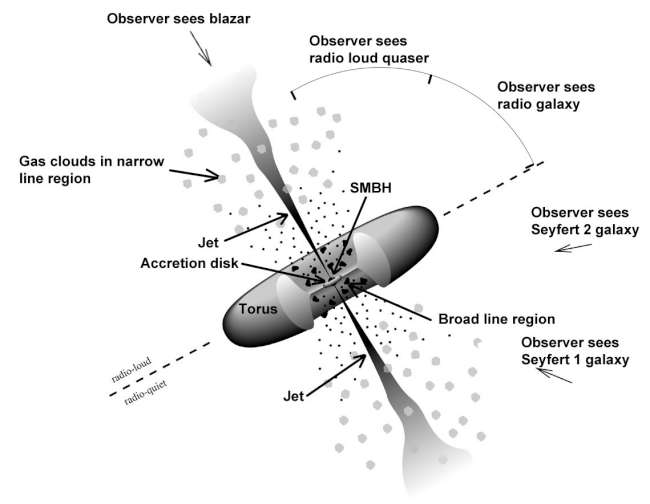
\includegraphics[width=\textwidth]{pictures/Chapter2/AGN_unified_model.jpg}
	\caption{Unification model of an AGN \parencite{fermi2025figure1}.}
	\label{fig:agn_sed}
\end{figure}



\subsection{Spectral Features}
\label{sec:spectral_features}

AGNs emit radiation across the entire electromagnetic spectrum. A typical AGN exhibits strong X-ray and radio emission, as well as non-stellar ultraviolet and optical continua, along with both broad and narrow emission lines. However, not every AGN displays all of these features, as will be discussed in more detail later \parencite{peterson1997introduction}.
\subsubsection{Non-stellar Continuum Emission}
AGNs typically have a strong, non-stellar continuum emission. In the optical and ultraviolet range, the spectrum often follows a power-law shape instead of a blackbody curve, which implies a non-thermal origin. A noticeable feature in this part of the spectrum is the so-called \emph{big blue bump}, a broad increase in emission that peaks in the ultraviolet between about 1000 and 3000\,\AA. It is thought to be caused by thermal radiation from the hot inner part of the accretion disk around the supermassive black hole \parencite{peterson1997introduction, osterbrock1989agn}. The shape and strength of this bump can give information about how fast matter is falling into the black hole. \\
Additionally, the ionized photons, emitted by the continuum, are responsible for exciting the gas clouds around the nucleus, which leads to emission lines in AGN spectra \parencite{osterbrock1989agn}.

\subsubsection{Broad Emission Lines}


\subsubsection{Narrow Emission Lines}


\subsubsection{Infrared Emission}


\subsubsection{X-ray Emission}


\subsubsection{Radio Emission}




\subsection{Variability}
\label{sec:variability}

\section{Reverberation Mapping}
\label{sec:reverberation_mapping}


\subsection{Principle}
\label{subsec:rm_principle}



The main focus of this work was to perform a classic reverberation analysis of NGC 4593, with a focus on the broad line region (BLR) and its geometry around the central supermassive black hole (SMBH).\\\\
This type of analysis aims to measure the time lag $\tau$ between the variable continuum and the emission line response, in order to determine the spatial scale and structure of the BLR. By observing these variations over time and analyzing the delayed response of the broad lines, it is possible to learn more about the geometry and dynamics of the BLR and to estimate the mass of the SMBH.\\\\
Reverberation mapping (RM) is based on the strong correlation between a variable continuum emission $C(t)$ and the emission line flux $L(\nu, t)$ \parencite{horne2021space}. This correlation originates from the photoionization of gas clouds in the BLR by the central continuum source. As the continuum changes, the emission lines react in a similar way, but with a time delay $\tau$, because of the distance between the central source and the BLR. This delay corresponds to the time it takes for light to travel from the central source to the BLR.\\\\

\subsection{Transferfunction}
\label{subsec:rm_transferfunction}

\subsection{Cross-Correlation Function}
\label{subsec:rm_ccf}

\subsection{Black-Hole Mass}
\label{subsec:rm_bh_mass}

\section{Bowen Fluorescence}
\label{sec:bowen_fluorescence}